\chapter{Analyse Statique : audit d'OpenSSL}

\section{But de cette partie}
Nous nous sommes concentrés sur les parties qui peuvent être critiques : 
\begin{description}
	\item [l'entropie :] un des problèmes les plus épineux lors de la génération de clef;
	\item [la génération des clefs : ] c'est sur elles que reposent une bonne partie de la sécurité. Si leur secret venait à être découvert, les fonctions de chiffrement ne servent plus à rien (il sont en théorie connus et éprouvés);
	\item [les chiffrements et leur protocole :] régulièrement, des failles sont trouvées dans ces protocoles, et les avancées technologiques poussent aussi à rendre des algorithme obsolètes (augmentation de la puissance de calcul des machines);
	\item [les signatures et leurs authentifications : ] parce que les certificats et les signatures électroniques sont bien plus présents qu'on ne pourrait le croire. Le mécanisme est souvent transparent à l'utilisateur, mais les certificats sont devenus indispensables;
	\item [les protocoles SSL et TLS : ] OpenSSL est basé directement sur le protocole SSL puis ensuite sur celui de TLS (successeur de SSL).\\
\end{description}
Cette deuxième partie est un très court résumé du rapport d'audit réalisé pendant le projet. Pour de plus amples informations, nous vous conseillons de le consulter.

\subsection{Entropie}

L'entropie est la base pour générer des nombres pseudo-aléatoire. Elle joue donc un rôle prépondérant dans la sécurité de la cryptographie qui sera mise en place. Son générateur est composé de trois principaux éléments : 
\begin{description}
	\item [le bruit source : ] il doit être non déterministe, et renvoie de façon aléatoire des bits grâce à des processus non déterministes;
	\item [le composant de conditionnement : ] il permet d’augmenter ou diminuer le taux d’entropie reçu;
	\item [une batterie de tests : ] elle fait partie également intégrante du système. Des tests sont réalisés pour déterminer l’état de santé du générateur aléatoire, permettant de s’assurer que la source d’entropie fonctionne comme attendu.\\
\end{description}

Plusieurs standards parlent de l'entropie, dont principalement la RFC 4086 \ref{rfc4086} et le FIPS 140 \ref{fips140-1} \ref{fips140-2}. Mais malgré les recommandations, quelques failles ont été trouvées. Pour plus d'informations, nous vous invitons à aller consulter le rapport d'audit.

\subsection{Génération des clefs}

Les clefs cryptographiques sont un principe fondamental en cryptographie. En effet, elles sont censées être le seul secret à garder précieusement par leur possesseurs : il est conseillé que les algorithmes et tous les outils ne soient pas secret afin d'être certain de ne pas insérer de faille. Les algorithme reconnus et éprouvés sont beaucoup plus fiables que les algorithmes secrets et personnels.\\

Par conséquent les clefs se doivent d'être les plus solides possible. Mais malgré le soin qu'on peut y apporter, et les différentes recommandations qui sont faites par les normes, des failles existent. Nous vous invitons à vous référer au rapport d'audit pour de plus amples informations.

\subsection{Chiffrement et protocoles}
De nombreux protocoles de chiffrement existent : 
\begin{itemize}
	\item symétrique :
	\begin {itemize}
		\item AES;
		\item Blowfish;
		\item DES, ou aujourd'hui le triple-DES;
		\item etc.\\
	\end{itemize}
	\item asymétrique : 
	\begin {itemize}
		\item DSA;
		\item El Gamal;
		\item RSA;
		\item etc.\\
	\end{itemize}
\end{itemize}

RSA étant l'un des algorithmes les plus utilisés en cryptographie asymétrique, et le temps nous ayant été limité, nous nous sommes concentrés dessus.\\
Cependant, RSA seul n'est plus d'une sécurité absolue. Il est combiné à OAEP, qui constitue une sorte de prétraitement à RSA lui même. Nous parlons de RSA-OAEP. Grâce à OAEP, un padding est rajouté avant l'application de RSA. La norme princiaple qui se charge des recommandations sur RSA est la PKCS\#1, qui a aussi le nom de RFC 3447 \ref{rfc3447} \ref{rfc3447_trad}.
Plusieurs failles ont été trouvées et suite à ces découvertes, des recommandations ont été faites. Pour de plus amples informations nous vous invitons à parcourir le rapport d'audit.

\subsection{Signature et chiffrement}
La signature électronique est de plus en plus utilisée de nos jours, de façon plus ou moins transparente. Un mécanisme cmplexe est mis en place derrière, avec toute une chaîne d'autorités de certification et de révocation des certificats. Ils permettent de faire un lien fiable entre la clef et son possesseur. Processus de signature : 
\begin{figure}[H]
\begin{center}
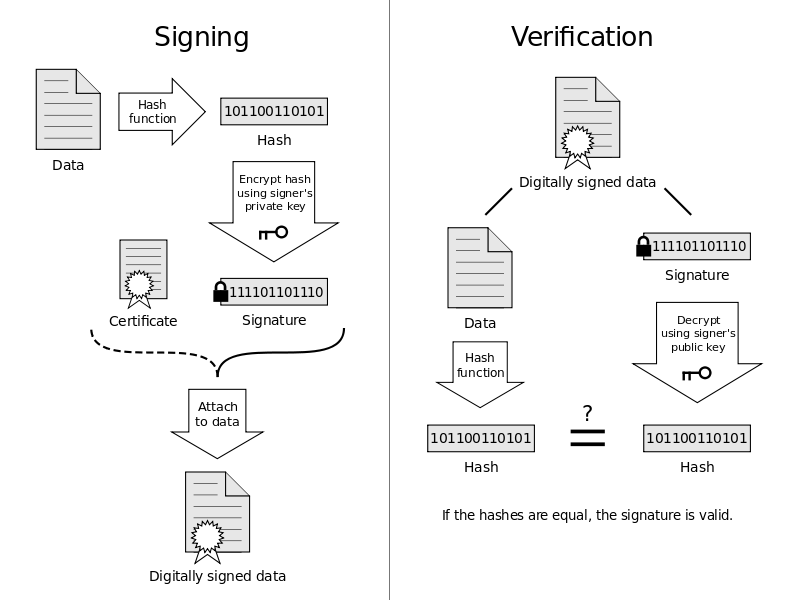
\includegraphics[width=10cm]{images/sig_dig.png}
\end{center}
\caption{Signature électronique}
\label{digital sig}
\end{figure}

La RFC 3447 \ref{rfc3447} \ref{rfc3447_trad} apporte aussi des recommandations à ce propos, ainsi que la RFC 979 \ref{rfc979}. Pour consulter les principales failles que nous avons trouvées à ce sujet, nous vous invitons à aller consulter le rapport d'audit.

\subsection{Protocole SSL/TLS}
SSL et TLS (successeur de SSL) sont des protocoles de sécurisation des échanges sur internet. Les versions 2 et 3 de SSL ont été développées par Netscape puis le brevet a été racheté par l’IETF en 2001 qui a publié une évolution de ce protocole en TLS. Ce protocole fonctionne selon un mode client-serveur et fournit les objectifs de sécurité suivants :
\begin{itemize}
	\item authentification serveur/client;
	\item confidentialité des données échangées;
	\item intégrité des données échangées.\\
\end{itemize}
Du point de vue réseau, ce protocole se situe dans la couche session du modèle OSI et entre transport et application dans le modèle TCP.

Pour de plus amples informations, nous vous invitons à aller consulter le rapport d'audit.



















